\subsection{Explicación del algoritmo realizado}

Para resolver el problema de CMF de forma exacta, generamos un algoritmo encargado de recorrer todas las posibles cliques del grafo de entrada con la estrategia de $Backtracking$. Esto se debe a que no hallamos ninguna caracterización particular que nos permitiera reducir el espacio de búsqueda de cliques tal que el algoritmo ignorara una cantidad asintótica de ellas. Luego, nuestra implementación genera todas las soluciones posibles siguiendo un orden lexicográfico para evitar repetirlas. Por ejemplo, la clique $k_{2}$ formada por los nodos \{1,2\} es la misma que se forma al elegir los nodos \{2,1\}. Por lo tanto, al representar los nodos como números y formar cliques respetando su orden lexicográfico, nos ahorramos realizar repeticiones como la mencionada. 

De este modo, nuestro algoritmo comienza generando todas las cliques que contienen al nodo de menor valor numérico que no haya sido utilizado y, en cada paso, selecciona una serie de candidatos a ser agregados a la clique actual hasta que no quede ninguno. Una vez alcanzada dicha instancia, el algoritmo retrocede quitando el último nodo agregado a la clique e insertando al próximo candidato, si es que existe. El orden lexicográfico se respeta al momento de elegir los candidatos ya que sólo pueden ser seleccionados como tales aquellos cuyo valor representativo sea mayor al del último nodo agregado a la clique.

A continuación, se expone el pseudocódigo del algoritmo mencionado:\\

\underline{Variables globales:} \textbf{Conj(nodo)} $cliqueMaxima$, \textbf{Entero} $fronteraMaxima$.\\

\begin{algorithm}[H]
	\SetAlgoLined
	\caption{Algoritmo Exacto}
	\KwIn{\textbf{Grafo} $g$}
	\KwOut{\textbf{Conj(nodo)} $clique$}

	\For{nodo $v$ en $g$}{
		\textbf{Sort}(adyacentes($v$))
	}
	\textbf{Conj(nodo)} $clique = \emptyset$\\
	\textbf{Conj(nodo)} $candidatos = $ nodos($g$)\\

	Backtracking($clique$, $candidatos$)\\

	\textbf{devuelvo} $cliqueMaxima$\\

\end{algorithm}

\begin{algorithm}[H]
	\SetAlgoLined
	\caption{Backtracking}
	\KwIn{\textbf{Conj(nodo)} $clique$, \textbf{Conj(nodo)} $candidatos$, \textbf{Grafo} $g$} %esto hay que ponerlo bien
	\KwOut{\textbf{Conj(nodo)} $clique$}

	\For{$c \in candidatos$}{
		\If{\textbf{frontera}($ clique \cup \{c\} $) $> fronteraMaxima$ }{
			$cliqueMaxima = clique \cup \{c\} $\\
			$fronteraMaxima = $frontera($clique \cup \{c\}$)\\
		}
		\If{\textbf{frontera}($ clique \cup \{c\} $) $>$ \textbf{frontera}($clique$)}{
			Backtracking($ clique \cup \{c\} $, calcularCandidatos($ clique \cup \{c\} $), $g$, $c$)\\
		}
	}
\end{algorithm}

\begin{algorithm}[H]
	\SetAlgoLined
	\caption{frontera}
	\KwIn{\textbf{Conj(nodo)} $clique$, \textbf{Grafo} $g$} %esto hay que ponerlo bien
	\KwOut{\textbf{Entero} $res$}

	$res = 0$\\
	\For{\textbf{nodo} $v \in nodos(g)$}{
		$res = res + (\#adyacentes(v) - (\#clique - 1))$\\
	}

	\textbf{devuelvo} $res$\\

\end{algorithm}

\begin{algorithm}[H]
	\SetAlgoLined
	\caption{calcularCandidatos}
	\KwIn{\textbf{Conj(nodo)} $clique$, \textbf{Grafo} $g$, \textbf{Nodo} $ultimoNodoAgregado$} %esto hay que ponerlo bien
	\KwOut{\textbf{Conj(nodo)} $candidatos$}

	nodo $w$ = elemento de la $clique$\\

	$candidatos = adyacentes(w)$\\
	\ForAll{$v \in nodos(g)$ con $v \neq w$}{
		$candidatos$ = interseccion entre $adyacentes(v)$ y $candidatos$\\
	}

	quitar de $candidatos$ todos los nodos de valor menor a $ultimoNodoAgregado$

	\textbf{devuelvo} $candidatos$\\

\end{algorithm}

Como operaciones preeliminares, el algoritmo ordena las aristas en su representacion interna del grafo. Esto permite hacer que ciertas operaciones tengan un costo temporal menor. Mas especificamente, hacer la interseccion entre los nodos adyacentes a dos nodos tiene un costo lineal siempre y cuadno los conjuntos esten ordenados.

Nuestro programa comienza con la función $Algoritmo\ Exacto$ que se encarga de inicializar los valores con los que se llama a $Backtracking$. A su vez, esta última realiza las llamadas recursivas necesarias para ir buscando las diferentes cliques y sus candidatos, teniendo en cuenta el orden lexicográfico mencionado anteriormente. Al realizar dicho procedimiento, el algoritmo verifica en cada paso que las cliques que va considerando sean mejores que la mejor encontrada hasta el momento. Si esto no ocurre, quita el nodo en cuestión y deja de explorar cliques conteniéndolo.\\
\newline
Por otra parte, la función $calcularCandidatos$ busca aquellos nodos no contenidos en la clique en exploración pero conectados con todos los que se encuentran en ella. Dicho procedimiento se logra encontrando la intersección entre todos los nodos adyacentes a los nodos de la clique mencionada.\\
\newline
Por otro lado, la función $frontera$ devuelve la cantidad de aristas de la frontera de una clique. Para efectuar dicho cálculo, se realiza la resta de la cantidad de nodos adyacentes a cada nodo de la clique menos la cantidad de nodos de ésta menos 1, lo que sería ($\forall v \in clique$) $\#adyacentes(v)-(\#nodos(clique)-1)$. La precondición de $frontera$ consiste en que los nodos del conjunto ingresado como parámetro sean todos adyacentes entre sí.

\subsection{Complejidad Temporal}

La complejidad temporal del algoritmo exacto realizado se encuentra acotada por la complejidad de la función de $Backtracking$ ya que el arbol de soluciones que toma el algoritmo implica revisar una cantidad de exponencial de opciones y esta cantidad es mayor a las demas funciones que haga el programa que son de orden polinomico, además el algoritmo entero encuentra su solucion llamando primero a la funcion $Backtracking$ lo cual significa que todo lo que suceda dentro de ella se multiplica por la cantidad de llamadas a $Backtracking$. Ésta se puede analizar a partir del árbol de soluciones del problema en cuestión, donde cada nodo representa a una clique cuya cantidad de nodos se encuentra determinada por el nivel en el que éste se ubica. Luego, la raíz es el único caso posible de 0 nodos, el primer nivel presenta todas las posibles cliques conteniendo un único nodo y así sucesivamente con todas las posibles combinaciones. Dado que buscamos cliques compuestas por 1 a $n$ nodos, encontrar las de tamaño $k$, con $k\leq n$, tiene un costo de $\mathcal{O}({n \choose k})$ = $\mathcal{O}(\frac{n!}{(n-k)!k!})$, siendo $\frac{n!}{(n-k)!k!} \leq n^k$. Por tanto, la cantidad de pasos de dicho procedimiento resulta $\sum\limits_{i=1}^n {n \choose i} = 2^n - 1$. 

Luego, podemos determinar que la complejidad de nuestro algoritmo exacto resulta $\mathcal{O}(2^n - 1) * \ costo\ de\ realizar\ cada\ paso$.

Veamos cuál es el costo de realizar cada paso:
\begin{itemize}
\item La función $calcularFrontera$ realiza un ciclo con la cantidad de nodos, en $\mathcal{O}(n)$, que es calculada con $size() (\mathcal{O}(1))$. En dicho ciclo, se le suma a un entero ($res$) el valor de un vector ($g$) al que se accede para, luego, acceder a otro ($nodos$) y se le resta 1 a este último. Esto se realiza en $\mathcal{O}(1)*\mathcal{O}(1)$ = $\mathcal{O}(1)$. Luego, la complejidad de dicha función resulta $\mathcal{O}(n)*\mathcal{O}(1)$ = $\mathcal{O}(n)$.
\item Por otro lado, la función $interseccionNAdyacentes$ comienza creando un vector ($v\_interseccion$), cuya complejidad temporal es $\mathcal{O}(n)$\footnote{http://www.cplusplus.com/reference/vector/vector/vector/} pues consiste en un constructor por copia, y un vector $v\_tmp$ por default en $\mathcal{O}(1)$. Luego, realiza un ciclo iterando la cantidad de nodos ($indices$) recibidos por parámetro, siendo $\#indices \leq n$. En dicho ciclo, ejecuta la función $set\_intersection$ ($\mathcal{O}(2*(n+n)-1)$ este costo reequiere que los conjuntos que van a ser intersecados esten ordenados en su representación interna, esto está garantizado al principio del algoritmo ordenando los vectores que representan a los nodos adyacentes de cada nodo. \footnote{http://www.cplusplus.com/reference/algorithm/set\_intersection/?kw=set\_intersection}). Para dicha ejecución, toma el primer y último elemento de $v\_intersection$ con $begin()$ ($\mathcal{O}(1)$\footnote{http://www.cplusplus.com/reference/vector/vector/begin/}) y $end()$ ($\mathcal{O}(1)$\footnote{http://www.cplusplus.com/reference/vector/vector/end/}), como también el $back\_inserter$ de $v\_temp$ ($\mathcal{O}(n)$) y el primer y último elemento del arreglo $g$ en la posicion $indices(i)$. Dado que éstos últimos son accesos a arreglos, se realizan en $\mathcal{O}(1)$. Luego, la complejidad temporal de dicho ciclo resulta $\mathcal{O}(n)*5\mathcal{O}(1)*\mathcal{O}(n)$ = $\mathcal{O}(n^2)$.\newline
\newline
Por otro lado, se crea una cola por default en $\mathcal{O}(1)$\footnote{//www.cplusplus.com/reference/queue/queue/queue/} y, luego, se llama a un nuevo ciclo que recorre el vector $v\_intersection$ (cuyo peor caso es $\mathcal{O}(n)$). Dentro de dicho ciclo, se realiza una comparación entre un elemento de $indices$ y uno de $v\_interseccion$ ($\mathcal{O}(1)$ pues los accesos son $\mathcal{O}(1)$ cada uno y la comparación es $\mathcal{O}(1)$). Por otro lado, se realiza también un $push()$ ($\mathcal{O}(n)$\footnote{//www.cplusplus.com/reference/queue/queue/push/}). Luego, la complejidad temporal de dicho ciclo resulta $\mathcal{O}(n)*\mathcal{O}(1)*\mathcal{O}(1)$ = $\mathcal{O}(n)$.\newline
\newline
Finalmente, podemos concluir que la complejidad temporal de la función $interseccionNAdyacentes$ es $\mathcal{O}(n^2)$.
\item La función $backtracking$ comienza con la asignación a un entero de la frontera de $clique$, utilizando la función $calcularFrontera$ ($\mathcal{O}(n)$).\newline
\newline
Luego, se procede revisando si la cola $candidatos$ se encuentra vacía ($empty()$\footnote{http://www.cplusplus.com/reference/queue/queue/empty/}), en cuyo caso se le suma uno al tamaño de $clique$ ($\mathcal{O}(n)$\footnote{http://www.cplusplus.com/reference/vector/vector/resize/}).\newline
\newline
Por último, la función realiza un ciclo que itera (siempre que $candidatos$ no sea vacío) asignándole a $clique(tamaño-1)$ una referencia al siguiente elemento de candidatos con $front()$ ($\mathcal{O}(1)$\footnote{http://www.cplusplus.com/reference/queue/queue/front/}) y luego popeando $candidatos$ con $pop()$ ($\mathcal{O}(1)$\footnote{http://www.cplusplus.com/reference/queue/queue/pop/}). También, se calcula nuevamente la frontera de $clique$ y se realiza una comparación entre ésta y un entero ($\mathcal{O}(1)$) que implica una serie de asignaciones a variables enteras. Por último, se compara dicha frontera con un entero y termina por llamar recursivamente a la función $backtracking$ con $interseccionNAdyacentes$ de la nueva $clique$ formada durante la ejecución. Dichas llamadas recursivas son las que elevan la complejidad temporal del algoritmo a $\mathcal{O}(2^n - 1)$ por lo mencionado anteriormente.
\item Finalmente, la función $exacto$ crea por default un vector y una cola ($\mathcal{O}(1)$) y ejecuta un ciclo con el tamaño de $g$ (cuyo peor caso es $n$) en el que ordena ($\mathcal{O}(nlog(n))$\footnote{http://www.cplusplus.com/reference/algorithm/sort/?kw=sort})
el primer y último elemento del $i$-ésimo elemento de $g$. Luego, realiza un $push()$ de $candidatos$.\newline
\newline
Por otra parte, llama a la función $backtracking$ ($\mathcal{O}(2^n - 1)$) y, finalmente, recorre la solución obtenida para devolverla.
\end{itemize}

Finalmente, podemos afirmar que la complejidad temporal de nuestro algoritmo exacto resulta $\mathcal{O}(2^n - 1) * (\mathcal{O}(n) + \mathcal{O}(n^2))$ = $\mathcal{O}((2^n - 1) * n^{2})$ = $\mathcal{O}(n^{2} 2^n)$.

\subsection{Experimentación}

Para las pruebas de complejidad empírica, utilizamos los tests aleatorios proporcionados por la cátedra. Las mediciones de tiempo en nanosegundos se realizaron con la función $high\ resolution\ clock$\footnote{http://en.cppreference.com/w/cpp/chrono/high\_resolution\_clock} de la librería $Chrono$ de $C++$. 

Las funciones de complejidad con las que se compararon nuestros gráficos de tiempo fueron ajustadas por algoritmos matemáticos (proporcionados por \textbf{sci davis}). Dichos algoritmos se encargaron de multiplicarle y sumarle constantes a las funciones con el fin de que éstas se ajustaran a nuestros resultados sin modificar el comportamiento de las funciones utilizadas para comparar.
	
\begin{figure}[H] %[h] Aqui [b] para button [t] para top
\begin{center}
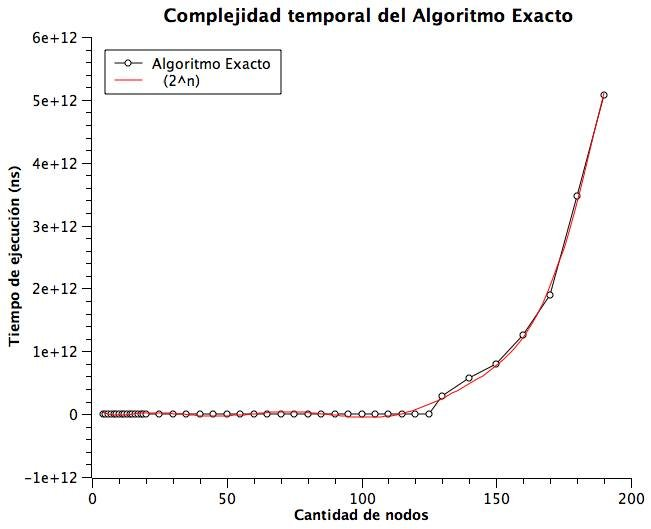
\includegraphics[width=350pt]{../imgs/exactoComplejidad.jpg}
\end{center}
\end{figure}

Como puede observarse en el gráfico anterior, la complejidad de nuestro algoritmo exacto se encuentra acotada por una función exponencial.



























